Ebben  fejezetben külön-külön bemutatom a helpdesk alkalmazást felépítő komponenseket. Kiemelem a komponensek által megvalósított funkciókat és a megvalósítás szempontjából fontos részleteket. 


\section{Mikroszerviz infrastruktúra}
A mikroszerviz specifikus funkciók megvalósításáért az itt bemutatott eszközök felelősek.

\subsection{Nginx}\label{sec:nginx}
Az Nginx-nek három különböző szerepe van:

\begin{itemize}
	\item a \foreignlanguage{british}{helpdesk frontend} alkalmazásszervereként működik (\ref{sec:angular}~pont),
	
	\item \foreignlanguage{british}{routing}ot valósít meg, rajta keresztül érhető el a \foreignlanguage{british}{helpdesk backend} és a \foreignlanguage{british}{Keycloak} szerviz,
	
	\item \foreignlanguage{british}{HTTP cache}-ként működik a frontend és a backend között.
\end{itemize}

A loadbalancer funkcionalitás --~mivel a docker azt natívan támogatja, így~-- a \foreignlanguage{british}{docker round-robin DNS}-én (\ref{sec:docker}) keresztül valósul meg.


\subsection{Docker konténerizáció}\label{sec:docker}
Az alakalmazás összes szolgáltatása saját docker konténerben fut. A docker konfigurációs leírása a \texttt{docker-compose.yml} állományban van. A \texttt{docker-compose} parancs ez alapján indítja el az alkalmazást, tölti le a szükséges \emph{image}-eket, hozza létre a saját alhálózatát, valósítja meg a hálózaton belüli DNS-funkciót.

A konténerek skálázása is a dockeren keresztül (\texttt{docker-compose ----scale}) valósul meg.


\subsection{Metrikák}\label{sec:metrikak}
\Aref{sec:metrikak_tervezes} pontnak megfelelően a springes alkalmazásaim egy-egy HTTP endpointon keresztül érhetőek el a Prometheus számára (\texttt{\mbox{/actuator/proemtheus}}) és induláskor beregisztrálják magukat az Eureka\footnote{Az Eureka a Netflix által fejlesztett \emph{discovery server}. Feladata az összes kliens port és ip adatának nyilkvántartása.} szerverbe.

A Prometheus az Eurekán keresztül találja meg az instance-eket, és 15 másodpercenként összegyűjti a metrikákat. Az alkalmazások információt küldenek a Kafka konnektoraikról, REST interfészeikről és az adatbázis kapcsolataikról\footnote{HikariCP-t használok JDBC kapcsolathoz}.

A Prometheus által összegyűjtött adatokat Grafanában létrehozott --~Spring Boot és JVM metrikákat tartalmazó~--   \emph{dashboard}okon ábrázolom.


\section{E-mail kliens}
Az e-mail kliens szerepe az üzenetek küldése és fogadása egy meghatározott e-mail címről. Feladata a külső protokollok leválasztása az alkalmazásról. Irányítja és karbantartja az IMAP és SMTP szerverrel való kapcsolatot.

\Aref{fig:email-client_sequence_diagram}. ábrán látható a két irányú kommunikáció megvalósulása:
\begin{itemize}
	\item az IMAP-on keresztül fogadott e-mailt az \texttt{email.in.v1.pub} kafka topicba írja,
	\item a saját --~e-mail cím specifikus~-- topic-jából kiolvassa az üzenetet és továbbítja  az SMTP szerver felé.
\end{itemize}


\begin{figure}[hbt] 
	\centering
	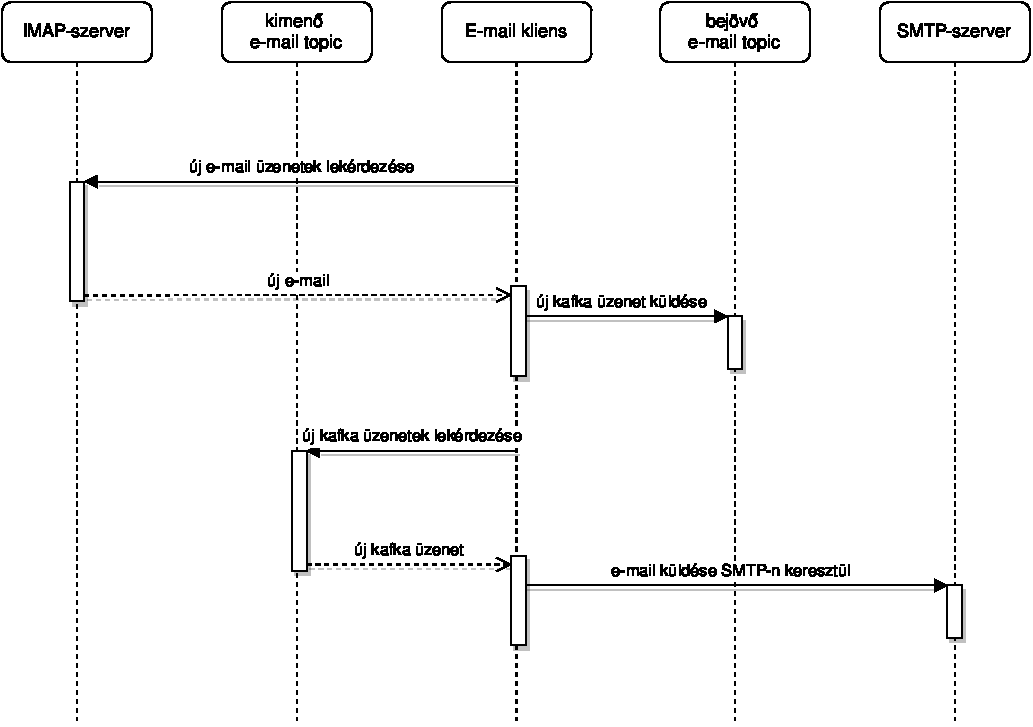
\includegraphics[width=0.85\textwidth]{email-client_sequence_diagram_drawio.pdf}
	\caption{E-mail kliens szekvencia diagramja}
	\label{fig:email-client_sequence_diagram}
	\floatfoot{Forrás: saját ábra}
\end{figure}




\subsection{E-mail szabvány}
Az elküldött üzenetek megfelelnek az \emph{rfc5322} szabványnak, különös tekintettel a 3.6.4. pontban~\cite{rfc5322_Identification_Fields} meghatározott mezőkre:

\begin{description}
	\item[Message-ID] egy globálisan egyedi azonosító ami egyértelműen azonosítja az üzenetet,
	
	\item[In-Reply-To] válasz esetén értéke eredeti üzenet \texttt{Message-ID}-ja,
	
	\item[References] azonosítja az üzenet szálat, értéke az eredeti üzenetek \texttt{Message-ID}-jai vesszővel elválasztva.
\end{description}

\subsection{Üzleti funkciók megvalósítása}
Az e-mail kliens fontosabb Java csomagjain keresztül bemutatom a forráskód felépítését, így betekintést nyújtva a megvalósított funkciókba.

\begin{description}
	\item[imap] csomag tartalmazza az IMAP protokoll megvalósításához szükséges kódrészleteket. A kapcsolat felépítéséért az \texttt{ImapMailReceiver}, míg az e-mailek fogadásáért az \texttt{EmailReceiver} osztály felelős. 
	
	\item[kafka] csomagba tartozó osztályok a \texttt{springframework.kafka} csomagja segítségével Kafka üzenetet küldenek (\texttt{EmailKafkaProducer} osztály) és fogadnak (\texttt{OutgoingEmailObserver} osztály).
	
	\item[smtp] csomagba tartozó \texttt{EmailSender} osztály a \texttt{springframework.mail} segítségével üzenetet küld az SMTP-szerveren keresztül.
\end{description}


\pagebreak
\section{Helpdesk backend}\label{sec:backend}
A backend felelős az e-mail szálakkal kapcsolatos üzleti feladatok ellátásáért. \Aref{fig:backend_sequence_diagram}. ábrán láthatóak a helpdesk backend funkciói:
\begin{itemize}
	\item fogadja és adatbázisban tárolja az \texttt{email.in.v1.pub} kafka topic-ból érkező e-maileket, 
	\item kiszolgálja a bejelentkezett felhasználók Nginx-en keresztül érkező kéréseit,
	\item válasz e-mail küldése esetén, adatbázisban tárolja, és a megfelelő kafka topic-ba írja az elküldendő üzeneteket,
	\item tárolja az e-mail szálakkal kapcsolatos adatokat.
\end{itemize}


\begin{figure}[hbt] 
	\centering
	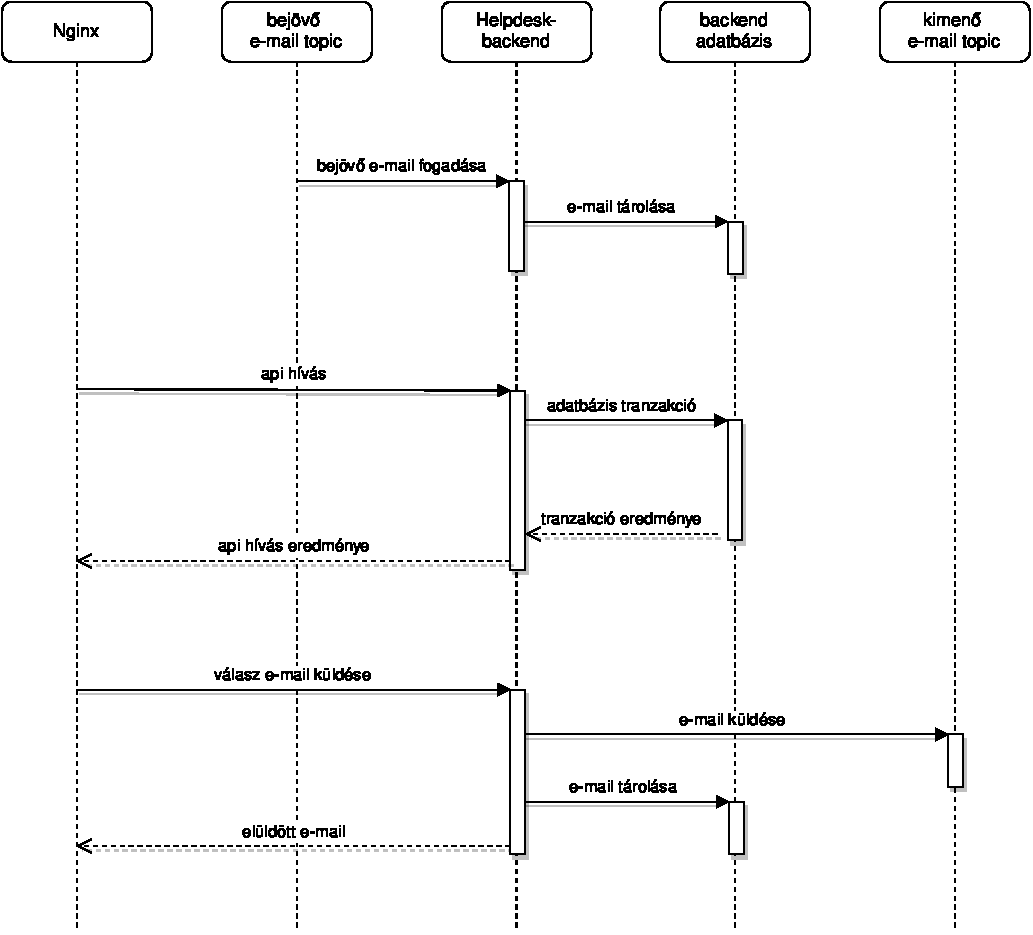
\includegraphics[width=0.85\textwidth]{backend_sequence_diagram_drawio.pdf}
	\caption{Helpdesk backend szekvencia diagramja}
	\label{fig:backend_sequence_diagram}
	\floatfoot{Forrás: saját ábra}
\end{figure}


\subsection{Spring Boot}
A forráskód a Spring Boot (\ref{sec:spring_boot} pont) keretrendszerrel készült. Az elérhető modulok közül a \emph{data-jpa}-t az adatbázis \texttt{repository}-jaihoz, a \emph{security}-t a keycloak integrációhoz, a \emph{web}et a \texttt{rest controller}ekhez, a \emph{micrometer}t és az \emph{actuator}t a metrikák elkészítéséhez használtam.	


\subsection{Adatbázis}\label{sec:adatbazis}
A Spring kezeli --~HikariCP-n keresztül~--   a PostgreSQL adatbázishoz való kapcsolódást.
Az adatok kezelését Hibernate-en (\ref{sec:JPA_implementacio_hibernate} pont) keresztül, az adatbázis verziókövetését Liquibase-en (\ref{sec:liquibase} pont) keresztül valósítom meg. 

Az e-mail szálak audit információinak és verzióinak követésére a Hibernate Envers (\ref{sec:hubernate_envers} pont) eszközét használom. Az Envers a neki létrehozott táblában automatikusan követi az annotációval megjelölt entitások állapotát.

\subsection{Pesszimista konkurenciakezelés}
Pesszimista konkurenciakezelésre jó példával szolgál a Liquibase (\ref{sec:liquibase} pont) működése. 

Minden indítás alkalmával a Liquibase --~az adatbázis módosításának befejezéséig~--   zárolja a \texttt{databasechangeloglock} táblát. Így --~a várakozás miatt~-- egyszerre mindig maximum egy Liquibase példány tud elindulni és módosításokat végrehajtani.


\subsection{Optimista konkurenciakezelés}
A \ref{sec:konkurencia_kezekese} pontban ismertetett optimista konkurenciakezelést az e-mail szálak módosítása során valósítja meg a backend.

A frontend kérésére egy verziószámmal ellátott e-mail szálat küld a backend. Ezt a HTTP-protokollnak megfelelő \texttt{eTag}-et a frontend megőrzi, majd a módosítások elvégzését követően --~mint \texttt{if-match} paraméter~-- visszaküldi a módosítási kérésével együtt.

A backend összehasonlítja a módosítani kívánt erőforrás verziószámát a kérésben érkezett \texttt{if-match} verziószámmal. Ha a két szám egyezik, akkor végrehajtja a változásokat, és az erőforrás új állapota új verziószámot kap.

Ha a két verzió nem egyezik --~ami csak úgy történhet meg, ha valaki más időközben módosította a kérdéses adatot~-- akkor a tranzakció nem hajtódik végre, és a kliens egy HTTP \texttt{Conflict} hibaüzenettel értesül a történtekről. A felhasználó ilyenkor az oldal frissítése után megvizsgálja az aktuális állapotot és --~amennyiben a módosításaira még mindig szükség van --~újból kezdi a folyamatot.

\subsection{Üzleti funkciók megvalósítása}
A backend által elvégzett feladatok bemutatása érdekében --~a legfontosabb csomagok ismertetésével~-- áttekintést adok a forráskód felépítéséről.


\begin{description}
	\item[kafka] csomagba a \texttt{springframework.kafka} csomagot használó, Kafka üzenetek kezelését végző osztályok tartoznak. Külön osztály foglalkozik a felhasználók (\texttt{UserObserver}) és az e-mailek (\texttt{IncomingEmailObserver}) fogadásával, és külön az e-mailek küldésével (\texttt{EmailKafkaProducer}).
	
	
	\item[security] a csomag feladata az alkalmazás HTTP protokollal kapcsolatos biztonsági paramétereinek beállítása. Itt lehet többek között a \emph{referrerPolicy}-t, \emph{CORS}-t és a jogosultság kezeléshez használt \emph{JSON Web Token} (\ref{sec:JWT}~pont) adatait megadni.
	
	
	\item[service] a csomagban az üzleti feladatok ellátásért felelős \texttt{service} interfészek és az azokat megvalósító osztályok találhatóak. Feladatuk az adatok üzleti szempontból lényeges tulajdonságainak ellenőrzése, valamint az üzleti logika végrehajtásához szükséges technikai feladatok delegálása. 
	

	\item[web.rest] csomagban találhatóak a \texttt{RestController}ek. A Spring ezeknek az osztályoknak továbbítja a REST kéréseket. Az osztályok fő célja a HTTP specifikus feladatok leválasztása az alkalmazásról, továbbá az üzleti igények továbbítása a megfelelő \texttt{service}-ek számára.	
\end{description}

Az \texttt{email-kliens}, a \texttt{keycloak-plugin} (lásd \aref{sec:backend_keycloak_separation}~pont), és a \texttt{helpdesk-backend} által közösen használt kódot --~a moduláris felépítés érdekében~-- külön, a \texttt{helpdesk-domain} maven projektben helyeztem el. A közösen használt modul legfontosabb csomagjait szintén itt mutatom be.


\begin{description}
	\item[dto] csomag nevét a \emph{Data Transfer Object} elnevezésről kapta. A csomag olyan érték osztályokat tartalmaz, amiknek nincs önálló viselkedésük, egyetlen feladatuk az adatok reprezentálása. Ezeknek a \texttt{dto}-k segítségével küldenek és fogadnak adatot a \texttt{RestController}ek.

	\item[entity] csomagban találhatóak a JPA entitások. Minden entitás osztály egy adatbázistábla Java oldali leképezése, és minden entitás objektum a tábla egy sorának a megfelelője. Az entitások állapotainak kezeléséért a Hibernate felel.
	
	\item[repository] csomagban a Spring \texttt{JpaRepository} interfészből öröklődő \texttt{repository} interfészek találhatóak. Feladatuk az adatbázisnak küldött utasítások reprezentálása. A szükséges SQL-t az interfészt implementáló Spring osztály hozza létre a metódus annotációjából vagy elnevezéséből~\cite{spring_boot_Query_Creation}.
	
	\item[mapper] csomagba tartozó osztályok feladata az adatok különböző reprezentációk --~\texttt{dto, entity, avro}~-- közötti leképezés megvalósítása. A \texttt{@Mapper} annotációival ellátott interfészek implementációját a Mapstruct (\ref{sec:retegek_szeparalasa}~pont) generálja fordítási időben.
	
	\item[avro] a Kafka üzenetekhez használt avro (lásd \ref{sec:apache_kafka}~pont) üzenetek Java reprezentációit a \texttt{hu.gdf.balazsbole.kafka} csomag tartalmazza. A csomagban található osztályokat fordítási időben az adatstruktúrát leíró \texttt{avdl} fájlból hozza létre az \texttt{avro-maven-plugin}.
\end{description}


\subsection{Egyéb eszközök}\label{sec:backend_egyeb_eszkozok}
A \texttt{DTO}-kban és az \texttt{entity}kben használt getter és setter  metódusok generálását a Lombok (\ref{sec:retegek_szeparalasa}~pont) segítségével végzem. A REST \texttt{endpoint}ok dokumentációját Swagger segítségével generálom. A Swagger a felannotált \texttt{dto} osztályokból és \texttt{RestController} metódusokból szabványos OpenApi dokumentációt készít. A dokumentációt \aref{appendix:openapi} függelékben csatoltam a dolgozatomhoz.



\section{Helpdesk frontend}
A frontend az e-mailek és e-mail szálakkal összefüggő üzleti feladatok megjelenítéséért felelős. A felhasználók jogosultság ellenőrzését végzi el, a bejelentkeztetésüket átirányítja a Keycloak szervernek. 


\subsection{Kommunikáció a backenddel}
A backenddel való kommunikáció HTTP protokollon keresztül zajlik, a szükséges \texttt{service} osztályokat az OpenApi dokumentációból (\ref{sec:backend_egyeb_eszkozok}) a \texttt{swagger angular generator} hozza létre.

Az aszinkron HTTP hívásokat az NgRx könyvtár alakítja adatfolyamokká. 
Az így \emph{Observable}-ként kezelt események már támogatják a stream műveleteket, megkönnyítik a filterezhetőséget és az egységes hibakezelést. 

Az NgRx használatával továbbá elkerülhetőek az aszinkron hívások mellékhatásai, és egy globális, alkalmazás szintű belső állapot hozható létre.

\subsection{Komponensek}
Az egységes megjelenés és az ismerős kinézet miatt a komponenseim alapjának az Angular Material UI könyvtárat választottam. A könyvtár népszerű az Angular fejlesztők körében, mert a leggyakrabban előforduló felhasználói igényekre elérhető benne kész, könnyen használható megoldás.

A válasz e-mail létrehozására a nyílt forráskódú Quill szövegszerkesztőt használtam, mert egyszerűen beilleszthető az Angular környezetbe, és a felhasználó számára intuitív kezelőfelülettel rendelkezik.

\subsection{Üzleti funkciók megvalósítása}\label{sec:frontend_uzleti_funkciok}
Az üzleti funkciók megvalósításának bemutatása érdekében ismertetem a helpdesk frontend menüjét és a menüpontok által megvalósított üzleti funkciókat.
\begin{description}
	\item[Reply] a menüpont minden felhasználónak elérhető. Segítségével az \textsc{open} státuszú üzenetszálak elolvashatóak --~az üzenetek olvasottnak és olvasatlannak jelölhetőek~-- és megválaszolhatóak.
	A válasz e-mail küldése során az üzenetszál új állapotra állítható.
	
	\item[Edit threads] a menüpont minden felhasználónak elérhető. Segítségével a felhasználóhoz tartozó \textsc{open}, \textsc{resolved} és \textsc{clarification} státuszú e-mail szálak szerkeszthetőek. Az üzenetszálak tulajdonos, státusz, valamint --~adminisztrátor jogkörrel rendelkező felhasználó esetén~-- sor tulajdonsága változtatható meg.
	
	\item[History] szintén minden felhasználó számára elérhető menüpont. Segítségével --~táblázatba rendezve~-- lekérdezhetőek és visszakereshetőek a bejelentkezett felhasználóval kapcsolatba került e-mail szálak tulajdonságainak korábbi változásai.		
	
	\item[Change queue] csak az adminisztrátor felhasználónak elérhető menüpont. A felhasználó aktuális sorához tartozó \textsc{change\textunderscore queue} státuszú e-mail szálak érhetőek el és módosíthatóak vele. A kiválasztott e-mail szál az \texttt{Edit~threads} menüponthoz hasonlóan szerkeszthető.
	
	
	\item[User account] minden felhasználónak elérhető. A menüpont a felhasználó Keycloak profil oldalára navigál. Az oldalon megváltoztathatóak a bejelentkezett felhasználó személyes adatai és jelszava, megtekinthetőek a jogosultságai és azonosítással kapcsolatos eseményei, valamint érvényteleníthetőek a munkamenetei.
	
	\item[Choose queue] a menüpont adminisztrátor felhasználónak többször is, minden más felhasználónak csak egyszer érhető el. Segítségével --~az aktív felhasználót~-- a rendelkezésre álló sorok valamelyikéhez lehet rendelni.
	
	\bigskip
	\item[Login service] minden felhasználónak megjelenő, de csak az konfigurációs jogkörrel rendelkező felhasználónak elérhető menüpont. Az elérhető funkciók leírását \aref{sec:keycloak} pont tartalmazza.
	
	\item[Spring metrics] \aref{sec:metrikak} pontban leírt Spring Boot metrikákat ábrázoló Grafana oldalra navigáló menüpont.
	
	\item[Backend metrics] hasonlóan a Grafan oldalra navigáló --~a JVM metrikákat tartalmazó~-- menüpont.

	\item[Eureka service discovery] \aref{sec:bemutatas_eureka} pontban részletesen bemutatott Eureka szolgáltatás oldalára navigáló menüpont. 
	
	\item[Kafka messages] mindenkinek megjelenő, a Kafka Topics UI oldalára navigáló menüpont. Részletes bemutatása \aref{sec:kafka_topics} pontban olvasható.
	
\end{description}


\subsection{Futtatási környezet}
A kész program egy egyszerű HTML, CSS és JavaScript állománnyá fordul. A körülbelül $1,5$~MB-nyi forráskódot elegendő a böngészőbe egyszer letölteni, onnantól a program a kliens oldalon fut (lásd \ref{fig:frontend_sequence_diagram} ábra). A backend felé induló REST kéréseket a webszerver (\ref{sec:nginx}) osztja szét a rendelkezésre álló példányok között.

A frontend működését, és függőségeit \aref{fig:frontend_sequence_diagram}. ábra tartalmazza.

\begin{figure}[hbp] 
	\centering
	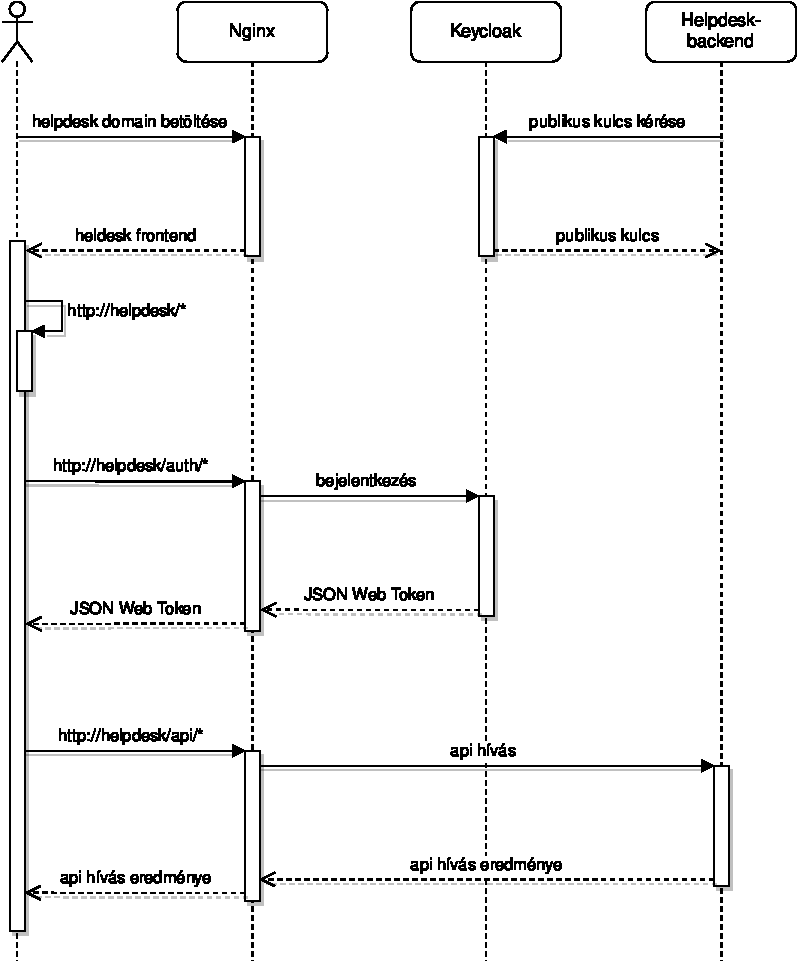
\includegraphics[width=0.85\textwidth]{frontend_sequence_diagram_drawio.pdf}
	\caption{Helpdesk frontend szekvencia diagramja}
	\label{fig:frontend_sequence_diagram}
	\floatfoot{Forrás: saját ábra}
\end{figure}

\pagebreak
\section{Keycloak}\label{sec:keycloak}
A Keycloak egy nyílt forráskódú jogosultság- és hozzáférés-kezelő. Támogatja az LDAP-ot, SSO-t és a kétlépcsős azonosítást~\cite{Keycloak_website}. 

A helpdesk alkalmazásban feladata a felhasználók azonosítása, és adataiknak nyilvántartása. Különálló mikroszervizként, saját adatbázissal rendelkezik.

Adminisztrátor felülete segítségével nyomon követhető a különböző autentikációhoz köthető események, szerkeszthetőek az aktuálisan érvényes szerepkörök, és --~hibakezelési céllal~-- megszemélyesíthetőek a felhasználók.


\subsection{Jogosultságkezelés}\label{sec:Jogosultságkezelés}
A jogosultságokat két eltérő területre osztottam fel. A \texttt{master realm} a regisztrációért és a jogkörök kiosztásáért, míg a \texttt{helpdesk realm} az alkalmazás funkcionális (\ref{sec:tobb_felhasznalo}) feladatiért felelős.

A \texttt{helpdesk realm}on belül további két jogkört különböztetek meg. Az \texttt{admin\textunderscore user} szerepbe tartozó felhasználók képesek más e-mail szálait is kezelni, míg a csupán \texttt{regular\textunderscore user} jogkörbe tartozóak csak a saját e-mail szálaikhoz férhetnek hozzá.


\subsection{JSON Web Token}\label{sec:JWT}
A jogosultságkezelés technikai alapját az \emph{rfc7519}-es szabványban~\cite{rfc7519_JSON_Web_Token} leírt JSON Web Token (JWT) adja. 

A Keycloak szervere által digitálisan aláírt \emph{acces\textunderscore token} (lásd \ref{sec:oauth_2_0}~pont) tartalmazza a felhasználó jogosultságait. A frontend minden HTTP lekérdezéshez csatolja ezt a Keycloaktól kapott azonosítót. A backend hitelesíti a tokent a Keycloak publikus kulcsával (lásd \ref{fig:frontend_sequence_diagram} ábra), és a megfelelő jogosultság megléte esetén engedélyezi a hozzáférést az erőforráshoz.

\subsection{OAuth 2.0 keretrendszer}\label{sec:oauth_2_0}
Mivel a Keycloak az ~emph{rfc7519}-es szabványban~\cite{rfc6749_OAuth_2_0} leírtaknak megfelelően állítja ki a jogosultságkezeléshez használt JSON Web Tokent, ezért Helpdesk Frontendnek ismernie kell, és a szabványban meghatározott módon szükséges az \emph{acces\textunderscore token}t kérvényeznie.

A Helpdesk Frontend az itt ismertetett módon kapja meg az \emph{acces\textunderscore token}t. A folyamat, az OAuth~2.0 jogosultságkezelő keretrendszernek megfelelően valósul meg.


\begin{enumerate}
	\item A Helpdesk Frontend a \emph{Login} gombra kattintva átirányítja a felhasználót a Key\-cloak regisztrációt és bejelentkezést kezelő oldalára. Az alkalmazás a kéréshez hozzáfűzi a Keycloak rendszerben tárolt kliensre jellemző azonosítót, belső állapotát és a --~harmadik lépésben~-- átirányításra használt webcímet.
	
	
	\item A Keycloak szerver megvizsgálja az egyes pontban kapott adatokat. Amennyiben a kérés a kliensazonosítónak megfelelő webcímről érkezett, az adatok pedig a klienshez regisztrált lehetséges értékekkel megegyeznek, akkor elkéri a felhasználó nevét és jelszavát. A szolgáltatás eldönti, hogy a megadott felhasználónév és jelszó alapján engedélyezhető-e a hozzáférés.
		
	
	\item Amennyiben a hozzáférés engedélyezhető, a szolgáltatás átirányítja a felhasználót az első pontban megadott webcímre, a címhez hozzáfűzi a négyes pontban használt hozzáférési kódot.
	
	 A \emph{Login} gomb a felhasználót a Frontend üdvözlő oldalára irányítja vissza.
	
	
	\item A Frontend a Keycloak szervertől HTTP POST metódussal kérvényezi az \emph{acces\textunderscore token}t. A lekérdezéssel elküldi az URL paraméterből kiolvasott hozzáférési kódot, a kliens azonosítót, és az egyes pontban használt átirányítási címet.
	
	
	\item A Keycloak ellenőrzi a hozzáférési kódot és megbizonyosodik arról, hogy az átirányítási cím megegyezik-e a hármas pontban használt címmel. Sikeres ellenőrzés után visszaküldi az \emph{acces\textunderscore token}t és a \emph{refresh\textunderscore token}t
	
	
	\item Az \emph{acces\textunderscore token} csupán 10 percig használható. Az idő lejárta után a Frontendnek új \emph{acces\textunderscore token}t kell igényelnie az előző pontban kapott \emph{refresh\textunderscore token} segítségével.
\end{enumerate}

A fent ismertetett folyamattal elérhető, hogy
\begin{itemize}
	\item az azonosításra használt érzékeny adatok --~az \emph{acces\textunderscore token} és a \emph{refresh\textunderscore token}~-- védetten, csupán a POST metódus paramétereként elérhetőek,
	
	\item a Helpdesk Frontendnek nem szükséges a felhasználó jelszavát kezelnie
	
	\item  és bejelentkezés illetve a regisztráció folyamata aszinkron módon történhet.
\end{itemize}


\section{Kafka}\label{sec:implementacio_kafka}
Annak érdekében, hogy teljesen elválasszam egymástól az e-mail klienst és a helpdesk backendet, a bejövő és kimenő e-mailek Kafka \emph{topic}-okon (\ref{sec:apache_kafka} pont) mennek keresztül. A szeparációval függetlenné teszem egymástól a két rendszer működését, ami lehetővé teszi az eltérő igénybevételnek (\ref{sec:granularitas} pont) megfelelő skálázhatóságot.

Ugyanígy, a funkciók szeparálása (\ref{sec:backend_keycloak_separation}) miatt a felhasználók adatai egy külön kafka topicban érhetőek el. Bármelyik mikroszerviznek szüksége lenne valamilyen felhasználóval kapcsolatos információra, azokat a topic végigolvasásával megkaphatja.



\section{Helpdesk backend és a Keycloak elkülönítése}\label{sec:backend_keycloak_separation}
A felhasználók adataiért a Keycloak (\ref{sec:keycloak}), az e-mail szálakért pedig a backend (\ref{sec:backend}) felelős. Az üzleti igény megköveteli hogy a felhasználók e-mail sorokhoz, és az e-mail szálak felhasználókhoz legyenek rendelve. A helpdesk backendnek éppen ezért tárolnia kell a fennálló kapcsolatokat.

A felhasználók a Keycloak felületén keresztül tudnak regisztrálni, és a személyes adataikat kezelni. A Keycloak által generált JSON Web Token (\ref{sec:JWT}) tartalmazza a felhasználók egyedi azonosítóját, a backendnek ezen az azonosítón keresztül kell a felhasználókat nyilvántartania és kiszolgálnia.

A felhasználók regisztrációja és adatainak változása --~\aref{sec:alkalmazasok_szeparalasa} pontban megismert CQRS útnak megfelelően~-- a \texttt{user.v1.pub} kafka (\ref{sec:implementacio_kafka}) topicban követhetőek nyomon.

A Keycloak Kafka integrációjának céljából hoztam létre a \texttt{keycloak-plugin} (\ref{fig:deployment_diagram} ábra) maven modult. A Keycloak eseményfigyelőként működő plugin, a megfigyelt eseményekről kafka üzenetet küld a kijelölt topicba. A helpdesk backend --~a topic üzeneteit olvasva~-- tartja karban a \texttt{users} táblát (\ref{fig:basic_database_uml}, \ref{fig:extended_database_uml} ábra). Így a helpdesk backend a felhasználókról mindig aktuális információval rendelkezik.

